%!TEX root = ../phd-thesis-lei-ma.tex
%!TeX spellcheck = en-US


\chapter{\label{chap:basics}General Principles of Neutrino Oscillations}

Because the flavor eigenstates of the neutrino are not the same as its propagation eigenstates, it can change flavor while it propagates.
In this chapter, I will use the two-flavor scheme to explain neutrino oscillations in some simple scenarios\footnote{In most physical problems, the two-flavor scheme is a good approximation to the phenomena of neutrino oscillations. The mass splits between the three mass eigenstates are so different that the corresponding oscillations occur on very different length scales. On the right length scale, the two-flavor scheme captures the prominent features of the neutrino oscillations of the corresponding mass split.}.
I will first discuss neutrino oscillations in vacuum. After explaining the general principles of neutrino oscillations in matter, I will show how the solar neutrino problem can be explained by neutrino oscillations. Finally, I will demonstrate the flavor isospin picture which can be used to visualize neutrino oscillations.


\section{\label{chap:basics-sec:vacuum-oscillations}Vacuum Oscillations}

Before working out the math, I can estimate the frequency of the oscillations of the neutrino between its flavors. In the natural units, frequency has the same dimension as energy (see Appendix~\ref{chap:app-sec:conventions-subsec:units}). Consider an electron neutrino with momentum $p$ which is a superposition of the two mass eigenstates $\ket{\nu_i}$ ($i=1,2$) with masses $m_i$, respectively. Since the neutrino masses are small, I can Taylor expand the energy of each mass eigenstate in terms of the corresponding mass:
\begin{align}
E_i & = \sqrt{m_i^2 + p^2 } \nonumber\\
& = p \sqrt{\frac{m_i^2}{p^2} + 1} \nonumber\\
& \approx p + \frac{1}{2} \frac{m_i^2}{p}.
\label{chap:basics-section:neutrinos-eqn:energy-taylor}
\end{align}
The first term in the above equation produces a global phase to the flavor wave function of the neutrino which does not affect neutrino flavor oscillations. The characteristic energy scale in the problem is the difference between the energies of the two mass eigenstates,
\begin{equation}
    \omega_{\mathrm v} =  \frac{m_2^2-m_1^2}{2E} = \frac{\delta m^2}{2E},
    \label{chap:basics-section:neutrinos-eqn:qualitative-method-frequency}
\end{equation}
which turns out to be the vacuum oscillation frequency. Here $E=p$ is approximately the energy of the neutrino.

To work out the exact solution, I will utilize the Schr\"{o}dinger equation. The wave function in flavor basis $\Psi^{(\ff)}$ is related to the wave function in mass basis $\Psi^{(\vv)}$ through a unitary mixing matrix $\mathsf U$,
\begin{equation}
\Psi^{(\mathrm f)} = \mathsf{U}\Psi^{(\vv)},
\label{chap:vacuum-eqn:wavefunction}
\end{equation}
where the upper indices ${}^{(\vv)}$ and ${}^{(\ff)}$ are used to denote the corresponding bases. The mixing matrix can be expressed using the vacuum mixing angle $\theta_{\vv}$,
\begin{equation}
\mathsf{U} = \begin{pmatrix} \cos\theta_\vv & \sin \theta_\vv \\ -\sin \theta_\vv & \cos \theta_\vv \end{pmatrix}.
\end{equation}
In vacuum mass basis, the neutrino has a free propagation Hamiltonian
\begin{equation}
\mathsf H^{(\vv)} = \begin{pmatrix} E_1 & 0 \\
0 & E_2
\end{pmatrix}.
\end{equation}
To the first order, the Hamiltonian becomes
\begin{align}
\mathsf H^{(\vv)} &\approx \frac{1}{2E} \begin{pmatrix}
m_1^2 & 0 \\
0 & m_2^2
\end{pmatrix} + E \mathsf{I} \nonumber \\
& =  \frac{1}{4E} \begin{pmatrix}
 - \delta m^2 & 0 \\
0 & \delta m^2
\end{pmatrix}  + \left(\frac{m_2^2 + m_1^2}{4E}  + E \right) \mathsf{I}.
\end{align}
Because a multiple of the identity matrix $\mathsf{I}$ only gives an global phase to the neutrino flavor wave function, I will neglect it from now on, and the vacuum Hamiltonian simplifies to
\begin{equation}
\mathsf H^{(\vv)} =  \frac{\delta m^2}{4E} \begin{pmatrix}
-1 & 0 \\
0 & 1
\end{pmatrix} = -\frac{\delta m^2}{4E} \sigma_3 = -\frac{\omega_{\vv}}{2}\sigma_3,
\end{equation}
where
\begin{align}
\sigma_1 &=  \begin{pmatrix}
0 & 1 \\
1 & 0
\end{pmatrix}, &\sigma_2 &=  \begin{pmatrix}
0 & -\ii \\
\ii & 0
\end{pmatrix},  &\sigma_3 &=  \begin{pmatrix}
1 & 0 \\
0 & -1
\end{pmatrix}
\end{align}
are the three Pauli matrices.
The Schr\"{o}dinger equation has the following simple solution in mass basis:
\begin{equation}
\Psi^{(\vv)}(t) = \begin{pmatrix}
c_1(0) e^{i \omega_\vv t/2 } \\
c_2(0) e^{ -i\omega_\vv t/2 }
\end{pmatrix}.
\end{equation}
% where the initial condition is
% \begin{equation}
% \Psi_v^{(v)}(0) = \begin{pmatrix}
% c_1(0) \\
% c_2(0)
% \end{pmatrix}.
% \end{equation}
Using Eqn.~\ref{chap:vacuum-eqn:wavefunction}, I obtain the wave function in flavor basis,
\begin{align}
\Psi^{(\ff)}(t) &= \mathsf{U}\Psi^{(\vv)}(t) \\
& = \begin{pmatrix} \cos\theta_\vv & \sin \theta_\vv \\ -\sin \theta_\vv & \cos \theta_\vv \end{pmatrix} \begin{pmatrix} c_1(0) e^{i\omega_\vv t/2 } \\
c_2(0) e^{ -i\omega_\vv t/2 }    \end{pmatrix} .
\label{chap:vacuum-eqn:wavefuncion-time}
\end{align}
Alternatively, I can also determine the Hamiltonian in flavor basis first, which is
%then solve the Sch\"{o}dinger equation. I will not show the steps here, however, the Hamiltonian in flavor basis is presented for future use,
\begin{equation}
\mathsf H^{(\ff)} = \mathsf U \mathsf H^{(\vv)} \mathsf U^\dagger = -\frac{\omega_\vv}{2}\cos 2\theta_\vv \sigma_3 + \frac{\omega_\vv}{2} \sin 2\theta_\vv \sigma_1.
    \label{chap:basics-sec:vacuum-osc-eqn:hamiltonian-vacuum}
\end{equation}
By solving the Schr\"{o}dinger equation in flavor basis, I will obtain the same wave function as in Eqn.~\ref{chap:vacuum-eqn:wavefuncion-time}.

%In many astrophysical neutrino sources such as the solar core, electron neutrinos are the most abundant. Thus the initial condition is usually assumed to be electron flavor in the calculation which leads to the survival probability of electron flavor
The probability for a neutrino emitted in the electron flavor at time $t=0$ to be detected as the electron flavor at a later time $t$ is
\begin{equation}
P(t) = 1-\sin^2(2\theta_\vv)\sin^2\left( \frac{\omega_\vv t}{2} \right).
\end{equation}
Since the neutrino travels with approximately the speed of light, the electron neutrino survival probability at a distance $r$ from the source is
\begin{equation}
P(r) =  1-\sin^2(2\theta_\vv)\sin^2\left( \frac{\omega_\vv}{2} r \right).
\label{chap:basics-eqn:vacuum-electron-probability}
\end{equation}
%An important parameter in vacuum oscillations is the oscillation length of the neutrino flavor conversion which is $1/\omega_\vv$.This confirms our qualitative method result in Eqn.~\ref{chap:basics-section:neutrinos-eqn:qualitative-method-frequency}.
I plot the above result in Fig.~\ref{chap:basics-section:neutrinos-fig:vacuum-2-flavor-osc} which clearly shows the oscillatory behavior. The oscillation length is determined by the characteristic energy scale $\omega_\vv$, which confirms our qualitative method result in Eqn.~\ref{chap:basics-section:neutrinos-eqn:qualitative-method-frequency}. The oscillation amplitude is determined by $\sin^2(2\theta_\vv)$.

\begin{figure}[htp]
    \centering
    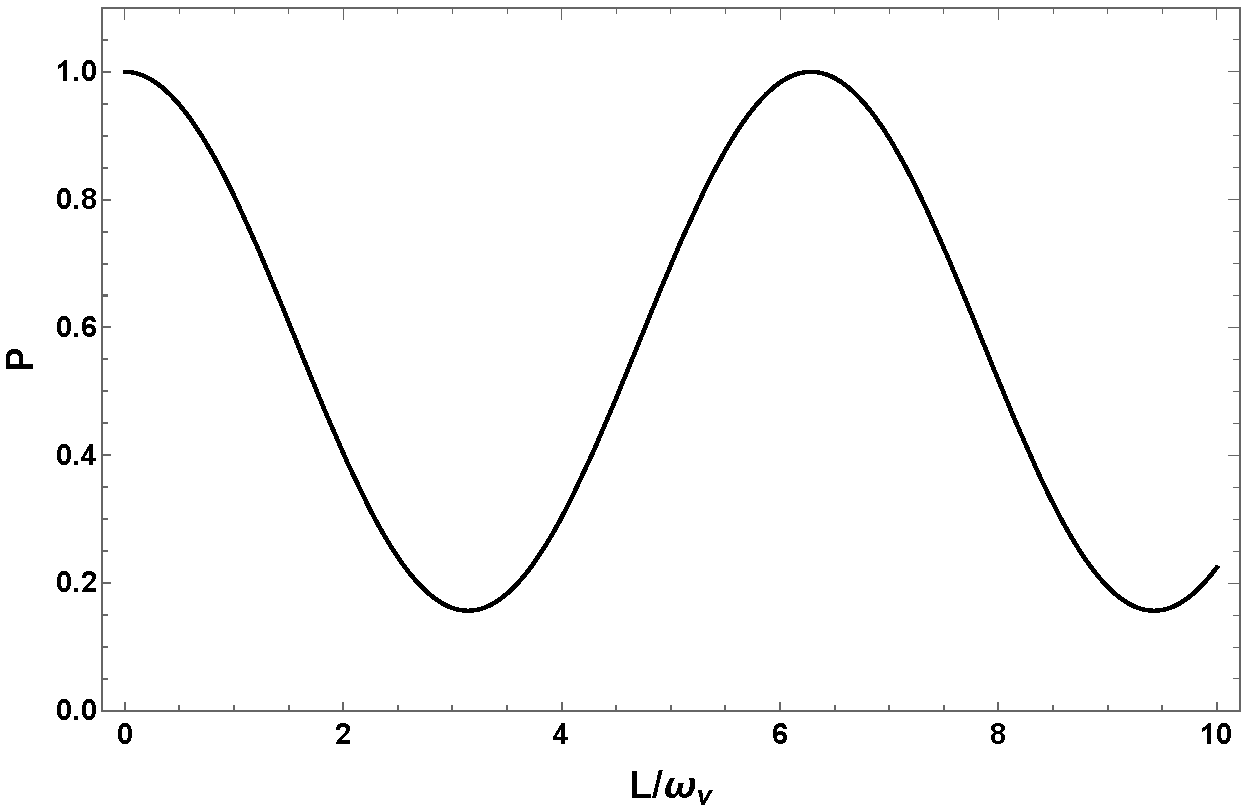
\includegraphics[width=0.8\textwidth]{chapters/assets/basics/neutrino-vaccum-osc-2-flavor.pdf}
    \caption{The electron flavor neutrino survival probability in vacuum oscillations as a function of distance $r$ which is measured in terms of vacuum oscillation frequency $\omega_\vv$. The mixing angle $\theta_\vv$ is given by $\sin^2\theta_\vv=0.30 \approx \sin^2 \theta_{12}$.}
    \label{chap:basics-section:neutrinos-fig:vacuum-2-flavor-osc}
\end{figure}



\begin{figure}[htp]
	\centering
	\begin{subfigure}[t]{0.48\textwidth}
		\centering
		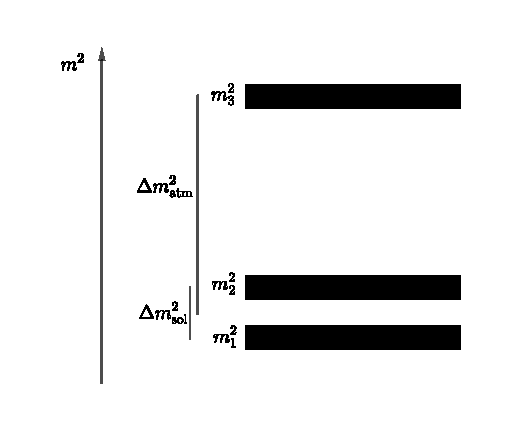
\includegraphics[width=\textwidth]{chapters/assets/basics/masses-nh}
		\caption{Normal hierarchy: the third mass is heavier than the first two.}
    \label{chap:basics-sec:flavor-isospin-pic-fig:masses-nh}
	\end{subfigure}
	\quad
	\begin{subfigure}[t]{0.48\textwidth}
		\centering
		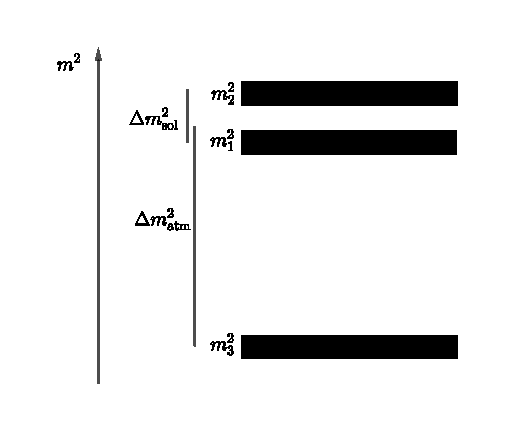
\includegraphics[width=\textwidth]{chapters/assets/basics/masses-ih}
		\caption{Inverted hierarchy: the third mass is smaller than the first two.}
    \label{chap:basics-sec:flavor-isospin-pic-fig:masses-ih}
	\end{subfigure}
	\caption{The order of the three neutrino masses. The difference between the first two masses is responsible for solar neutrino oscillations, and the difference between the third mass and the first two is responsible for atmospheric neutrino oscillations.}
    \label{chap:basics-sec:flavor-isospin-pic-fig:masses}
\end{figure}

\begin{figure}[htbp]
    \centering
    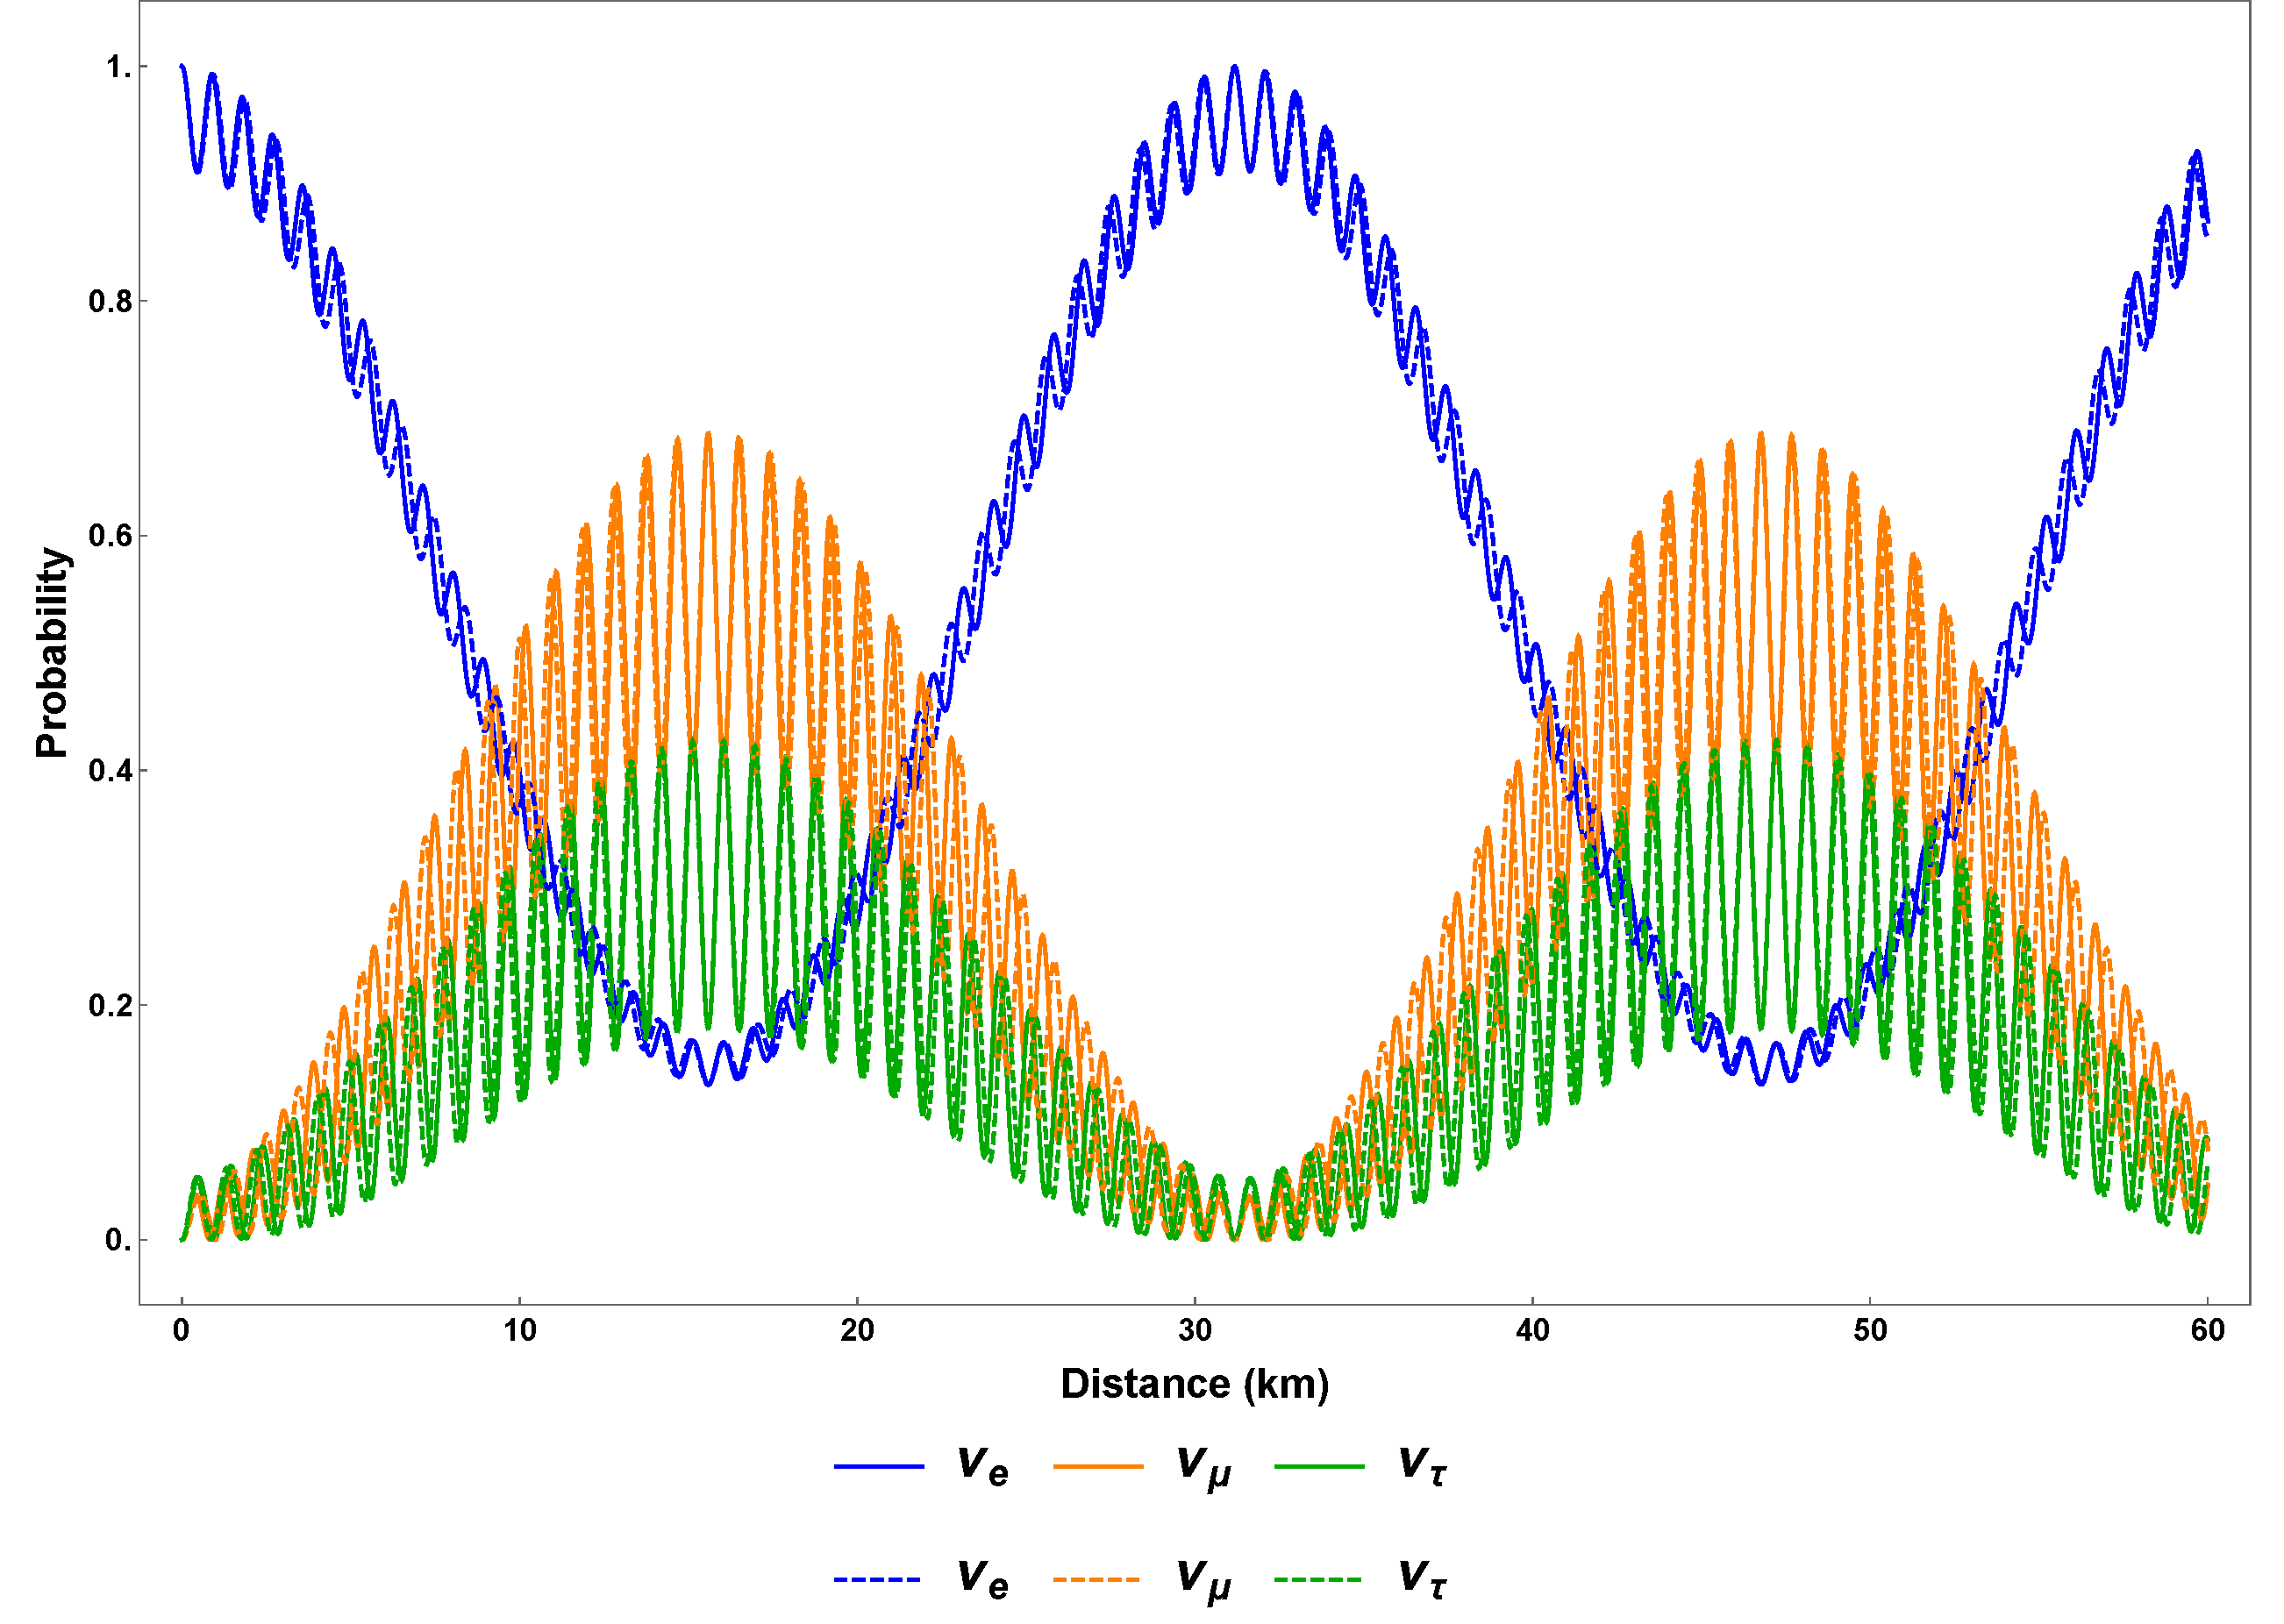
\includegraphics[width=\textwidth]{chapters/assets/basics/vacuum-oscillations-3-flavor.pdf}
    \caption{The probabilities for a $1\mathrm{MeV}$ neutrino, which is in the electron flavor initially, in different flavors as functions of the distance in vacuum. The solid lines represent the normal hierarchy and the dashed lines represent the inverted hierarchy. The mixing angles are $\sin^2\theta_{12}=0.30$, $\sin^2\theta_{13}=0.023$, and $\sin^2\theta_{23}=0.41$, respectively, and the mass differences are $\delta m_{21}^2 = 7.9\times 10^{-5}\mathrm{eV^2}$ and $\delta m^2_{23}=2.7\times 10^{-3}\mathrm{eV^2}$.}
    \label{chap:basics-section:neutrinos-fig:vacuum-3-flavor-osc}
\end{figure}


In nature, there are three neutrino flavors and, correspondingly, three neutrino mass eigenstates, which are shown in Fig.~\ref{chap:basics-sec:flavor-isospin-pic-fig:masses}. Because there are two different characteristic energy scales, $\omega_{\vv,21}=\delta m_{21}^2/2E$ and $\omega_{\vv,32}=\delta m_{31}^2/2E$, two oscillation periods should occur, as shown in Fig.~\ref{chap:basics-section:neutrinos-fig:vacuum-3-flavor-osc}. The fast oscillations are determined by the larger energy scale, $\omega_{\vv,32}$, while the slow oscillations are determined by the smaller one $\omega_{\vv,21}$. For the inverted neutrino mass hierarchy (with $m_3 < m_1 < m_2$), the oscillation frequencies are the same as in the normal mass hierarchy (with $m_3>m_2>m_1$) since they have the same characteristic energy scales. However, they will develop different phases during oscillations.

\clearpage

\section{\label{chap:basics-sec:oscillations-matter}Neutrino Oscillations in Matter}

\begin{figure}[htbp]
\centering
	\begin{subfigure}[t]{0.40\textwidth}
		\centering
		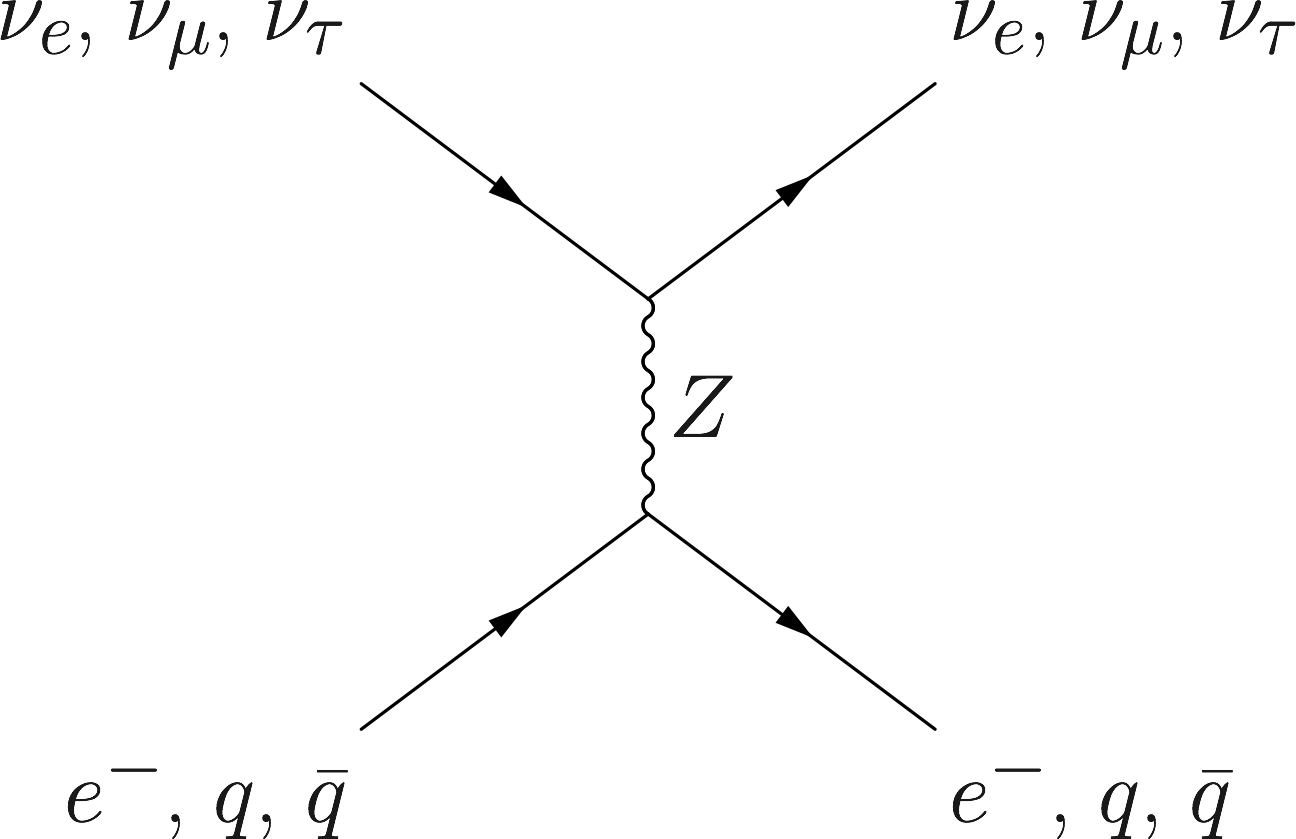
\includegraphics[height=0.2\textheight]{chapters/assets/matter/neutral-current.png}
    \caption{  }
		% \caption{Neutral current interaction between $\nu_{\mathrm e}$, $\nu_{\mu}$, $\nu_{\tau}$, and $e^{-}$. Neutral current interaction is mediated by Z bosons.}
    \label{chap:matter-fig:nc}
	\end{subfigure}%
  \qquad
	\begin{subfigure}[t]{0.40\textwidth}
		\centering
		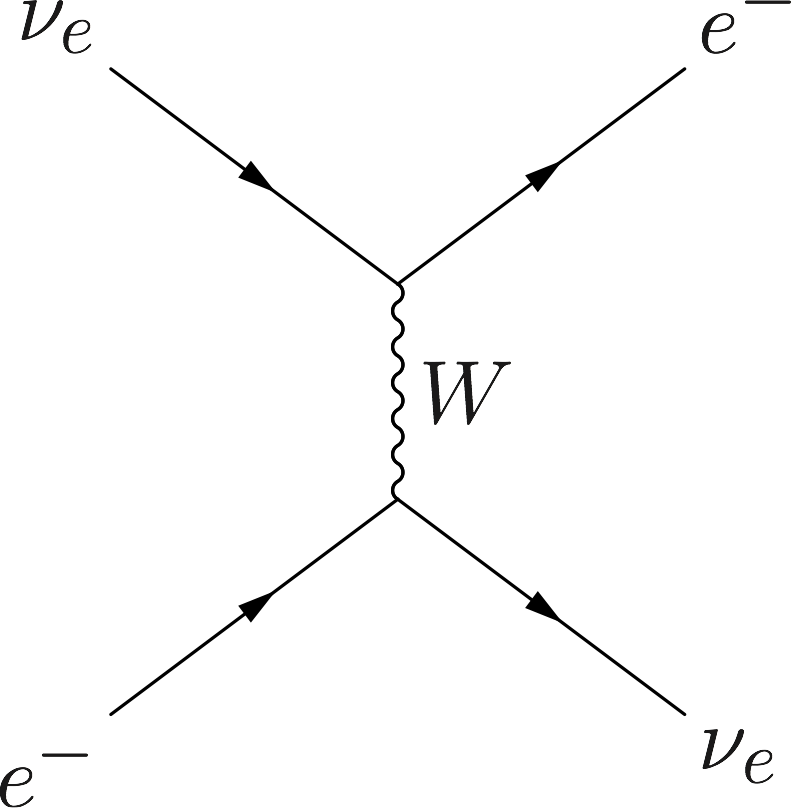
\includegraphics[height=0.2\textheight]{chapters/assets/matter/charged-current.png}
    \caption{  }
		% \caption{charged current interaction between $\nu_{\mathrm e}$ and $e^{-}$. Charged current interaction is mediated by W bosons.}
    \label{chap:matter-fig:cc}
	\end{subfigure}
	\caption{
  (a) The neutral current weak interaction does not distinguish between neutrino flavors and has no impact on neutrino oscillations. (b) The electron flavor neutrino acquires a unique refractive index contribution from the charged current weak interaction with ambient electrons.
  }
    \label{chap:matter-fig:nc-cc}
\end{figure}

In many astrophysical environments, such as stars and core-collapse supernovae, neutrinos are mostly produced at the center of the object and propagate through the dense matter envelope. Although this matter envelope is essentially transparent to neutrinos, the refractive indices of the neutrinos in matter are different than those in vacuum.\footnote{The word ``matter" in this disseration refers to ordinary matter composed of electrons, positrons, nucleons and nuclei. We assume that the temperature and density of the environment are not high enough to produce muons and tau particles. We will discuss the effect of dense neutrino medium in Chapter~\ref{chap:collective}.} Because the neutral current weak interaction does not distinguish between neutrino flavors (see Fig.~\ref{chap:matter-fig:nc}), it has no impact on neutrino oscillations, and I will ignore it from now on. Meanwhile, the electrons and positrons in matter will cause electron flavor neutrinos to have refractive indices different than other neutrino flavors through the charged current weak interaction (see Fig.~\ref{chap:matter-fig:cc}).
% One of the significant matter effect on neutrino flavor oscillations is the Mikheyev-Smirnov-Wolfenstein (MSW) effect~\cite{Mikheev:1986gs,wolf78,wolfensteinprd1979}, which is used to explain the deficit of electron flavor neutrino flux, as know as the solar neutrino problem~\cite{kuo1989,Petcov2002}. Later developments on the theories of matter effect revealed the parametric resonance of neutrino flavor oscillations due to fluctuations in matter density~\cite{Krastev1989,Akhmedov2000}, which is the neutrino analog of transitions between energy levels as a result of external optical stimulation. Parametric resonance is different from the MSW effect since it involves the parameters of the matter density, which is usually the period of matter density fluctuations. It has also be shown that neutrinos passing through the Earth can experience parametric resonance~\cite{Akhmedov1999, Petcov1998b}.
%Flavor conversion occurs as long as their propagation eigenstates are different from their flavor eigenstates. Since the neutral current interactions between the neutrinos and the matter is independent of the flavors, as shown in Fig.~\ref{chap:matter-fig:nc}, I only include the charged current interactions in the Hamiltonian, which is an effective potential for electron flavor.
This leads to an effective potential
\begin{equation}
\mathsf V^{(\ff)} = \frac{\sqrt{2}G_{\mathrm F} n_{\mathrm e} }{2}  \sigma_3,
\label{chap:basics-sec:oscillations-matter-eqn:effective-pot}
\end{equation}
where $G_{\mathrm F}$ is Fermi constant and $n_{\mathrm e}$ is net number density of the electron. As usual, I have ignored the trace terms in the above equation.

The Hamiltonian with the matter effect is the combination of Eqn.~\ref{chap:basics-sec:vacuum-osc-eqn:hamiltonian-vacuum} and Eqn.~\ref{chap:basics-sec:oscillations-matter-eqn:effective-pot}:
% \begin{equation}
% \mathsf H^{(\ff)} = \frac{ \omega_\vv }{2}\begin{pmatrix} -\cos 2\theta_\vv & \sin 2 \theta_\vv \\ \sin 2\theta_\vv & \cos 2\theta_\vv  \end{pmatrix},
% \end{equation}
% where we used the result of flavor basis vacuum oscillation Hamiltonian
% \begin{align}
% \mathsf H_\vv^{(\ff)}& = \mathsf{U} \mathsf H_\vv \mathsf{U}^\dagger \\
% &= \frac{ \omega_\vv }{2}\begin{pmatrix} -\cos 2\theta_\vv & \sin 2 \theta_\vv \\ \sin 2\theta_\vv & \cos 2\theta_\vv  \end{pmatrix}.
% \end{align}
\begin{equation}
\mathsf H^{(\ff)} = \left(\frac{\lambda}{2} -\frac{ \omega_\vv }{2} \cos 2\theta_\vv \right) {\sigma}_3  + \frac{ \omega_\vv }{2} \sin 2\theta_\vv {\sigma}_1,
\label{chap:basics-sec:msw-eqn:hamiltonian-matter-effect}
\end{equation}
where
\begin{equation}
  \lambda = \sqrt{2}G_{\mathrm F} n_{\mathrm e}.
  \label{chap:basics-sec:oscillations-matter-eqn:lambda}
\end{equation}
Due to the off-diagonal terms in $\mathsf H^{(\ff)}$, the neutrino will experience oscillations in flavor. A resonance with the maximum flavor mixing occurs when the diagonal terms of $\mathsf H^{(\ff)}$ vanish,
\begin{equation}
\frac{\lambda}{2} -\frac{ \omega }{2} \cos 2\theta_\vv  = 0,
\end{equation}
which gives the Mikheyev--Smirnov--Wolfenstein (MSW) resonance condition.


\section{\label{chap:matter-sec:solar-neutrinos}Neutrino Oscillations in the Sun}


% \section{\label{chap:basics-sec:msw}Mikheyev--Smirnov--Wolfenstein Effect}

The neutrinos produced in the solar core experience decreasing matter density as they travel outward through the Sun. The neutrino propagation eigenstates are different from the flavor states in general~\cite{wolf78}.
%The importance of matter effect to our understanding of solar neutrinos is that it modifies the oscillations, depending on the matter density variation.
Because the density change inside the Sun is not dramatic, the flavor quantum states of the neutrinos will evolve adiabatically inside the Sun.

\begin{figure}[htbp]
\centering
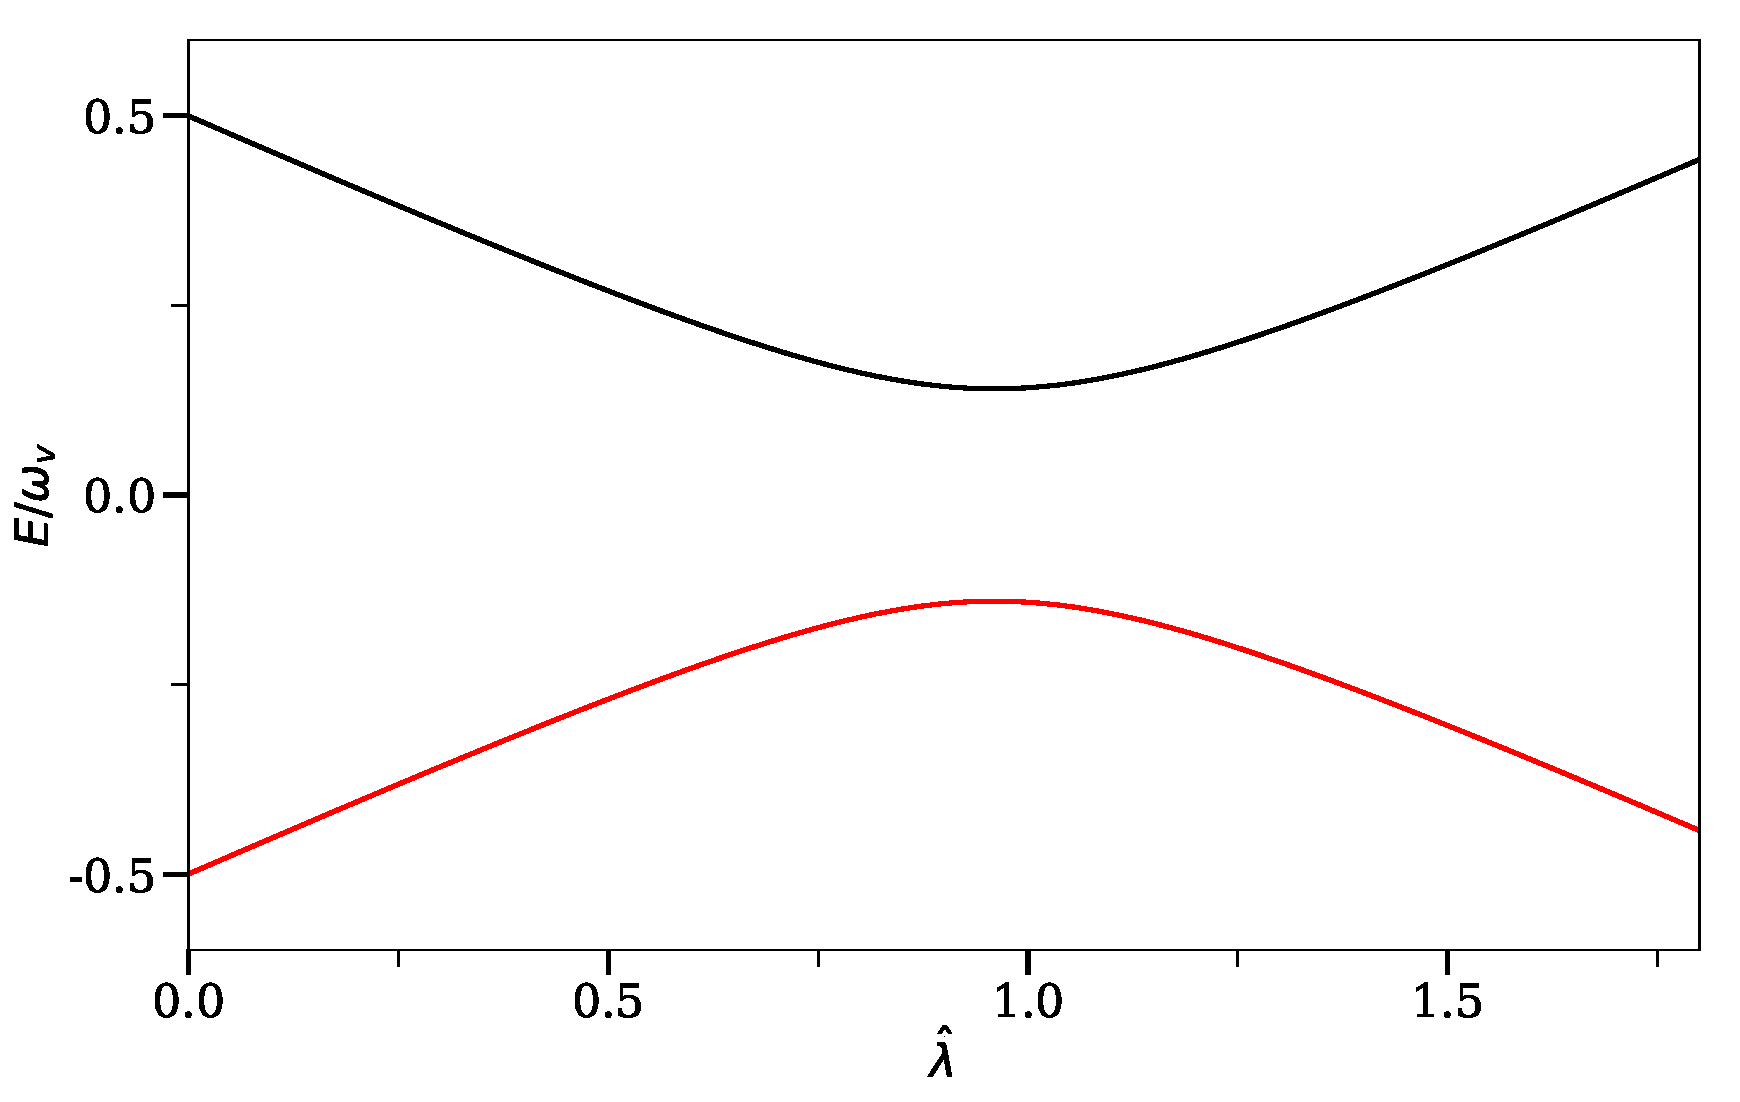
\includegraphics[width=0.7\columnwidth]{chapters/assets/matter/mswEnergyLevels}
\caption{The two eigenvalues of the neutrino Hamiltonian as functions of matter potential $\hat\lambda$. I have used $\sin^2\theta_\vv = 0.02 \approx \sin^2 \theta_{13}$.}
\label{fig:mswEnergyLevels}
\end{figure}

The values of the instantaneous eigenstates of the Hamiltonian, known as the heavy and light states, are
\begin{align}
\varepsilon_{\mathrm H} &= \frac{\omega_\vv}{2}\sqrt{ \hat\lambda +1 -  2\hat\lambda \cos 2\theta_\vv }, \\
\varepsilon_{\mathrm L} &= -\frac{\omega_\vv}{2}\sqrt{ \hat\lambda +1 -  2\hat\lambda \cos 2\theta_\vv },
\end{align}
% which means that the instantaneous eigenstates and eigenvectors of Hamiltonian is good enough for the time dependent Schr\"{o}dinger equation.
where
\begin{align}
\hat\lambda & = \frac{\lambda}{\omega_\vv}.
\end{align}
In Fig.~\ref{fig:mswEnergyLevels}, I show the two eigenvalues of the neutrino Hamiltonian as functions of the matter potential $\hat \lambda$.

For a very high matter density, the heavy state of the neutrino $\ket{\nu_{\mathrm H}}$ is almost the same as $\ket{\nu_{\ee}}$. As the matter density decreases, $\ket{\nu_{\mathrm H}}$ becomes a mixture of different neutrino flavors. As the neutrino reaches the surface of the Sun, where the matter density is approximately zero, $\ket{\nu_{\mathrm H}}$ is about the same as vacuum mass eigenstate $\ket{\nu_{2}}$. As a result, the electron flavor neutrinos produced at the solar core are partially converted to other flavors as they reach the surface of the Sun. This explains the solar neutrino problem.
% The MSW resonance occurs at $n_{\mathrm e} = 2\omega_\vv \cos(2\theta_\vv)/\sqrt{2}G_{\mathrm F}$.
%Neutrinos with different energies will encounter the MSW resonance at different matter densities, which will significantly reshape the neutrino energy spectra.
% Even though only the electron flavor neutrinos are produced in the Sun, the neutrino flavor conversion to the other flavors is enhanced by the matter interactions, in addition to the vacuum oscillation.
%The exact neutrino flavor conversion is much more complicated than the MSW effect.
% As an approximation, the MSW transition is good enough for the solar neutrinos flavor oscillations~\cite{Lopes2013a}.

% One of the interesting fact about MSW effect is the MSW triangle shown in Fig.~\ref{chap:basics-sec:msw-fig:msw-triangle}. The survival probability of the electron flavor neutrinos is plotted against $\log (\lambda/\omega_\vv)$ and $\log (\sin^2 2\theta_\vv)$. Qualitatively speaking, large conversion happens when matter density is not too small since a sufficient central potential is required for the level crossing. This leads to the triangle shape of the low survival probability region.
%
% \begin{figure}[htbp]
%     \centering
%     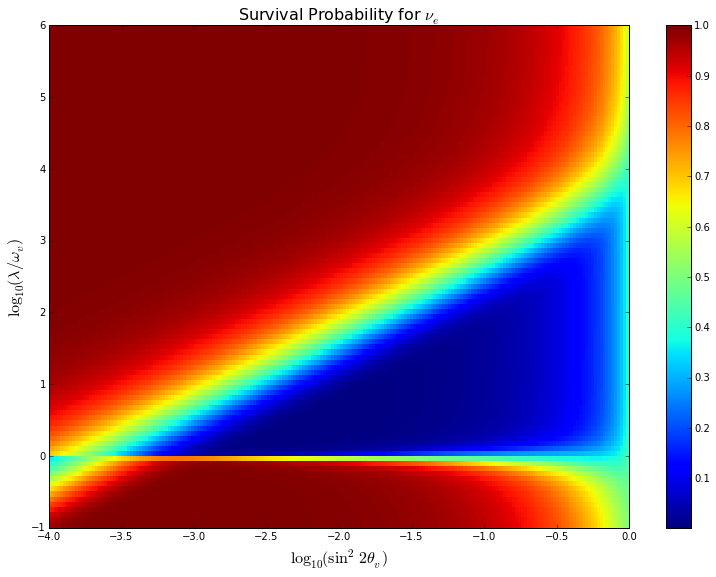
\includegraphics[width=0.9\textwidth]{chapters/assets/basics/msw-triangle.png}
%     \caption{MSW triangle. The horizontal axis is related to the the mixing angles, and the vertical axis is related to the matter potential in the center of the Sun. The colors are the survival probabilities of electron flavor. The region of large conversions, or small survival probabilities, forms a triangle. The larger the mixing angle, the larger range of matter potential for large conversions.}
%     \label{chap:basics-sec:msw-fig:msw-triangle}
% \end{figure}





% \section{\label{chap:matter-sec:flavor-isospin}Flavor Isospin Formalism}



\begin{figure}[htbp]
    \centering
    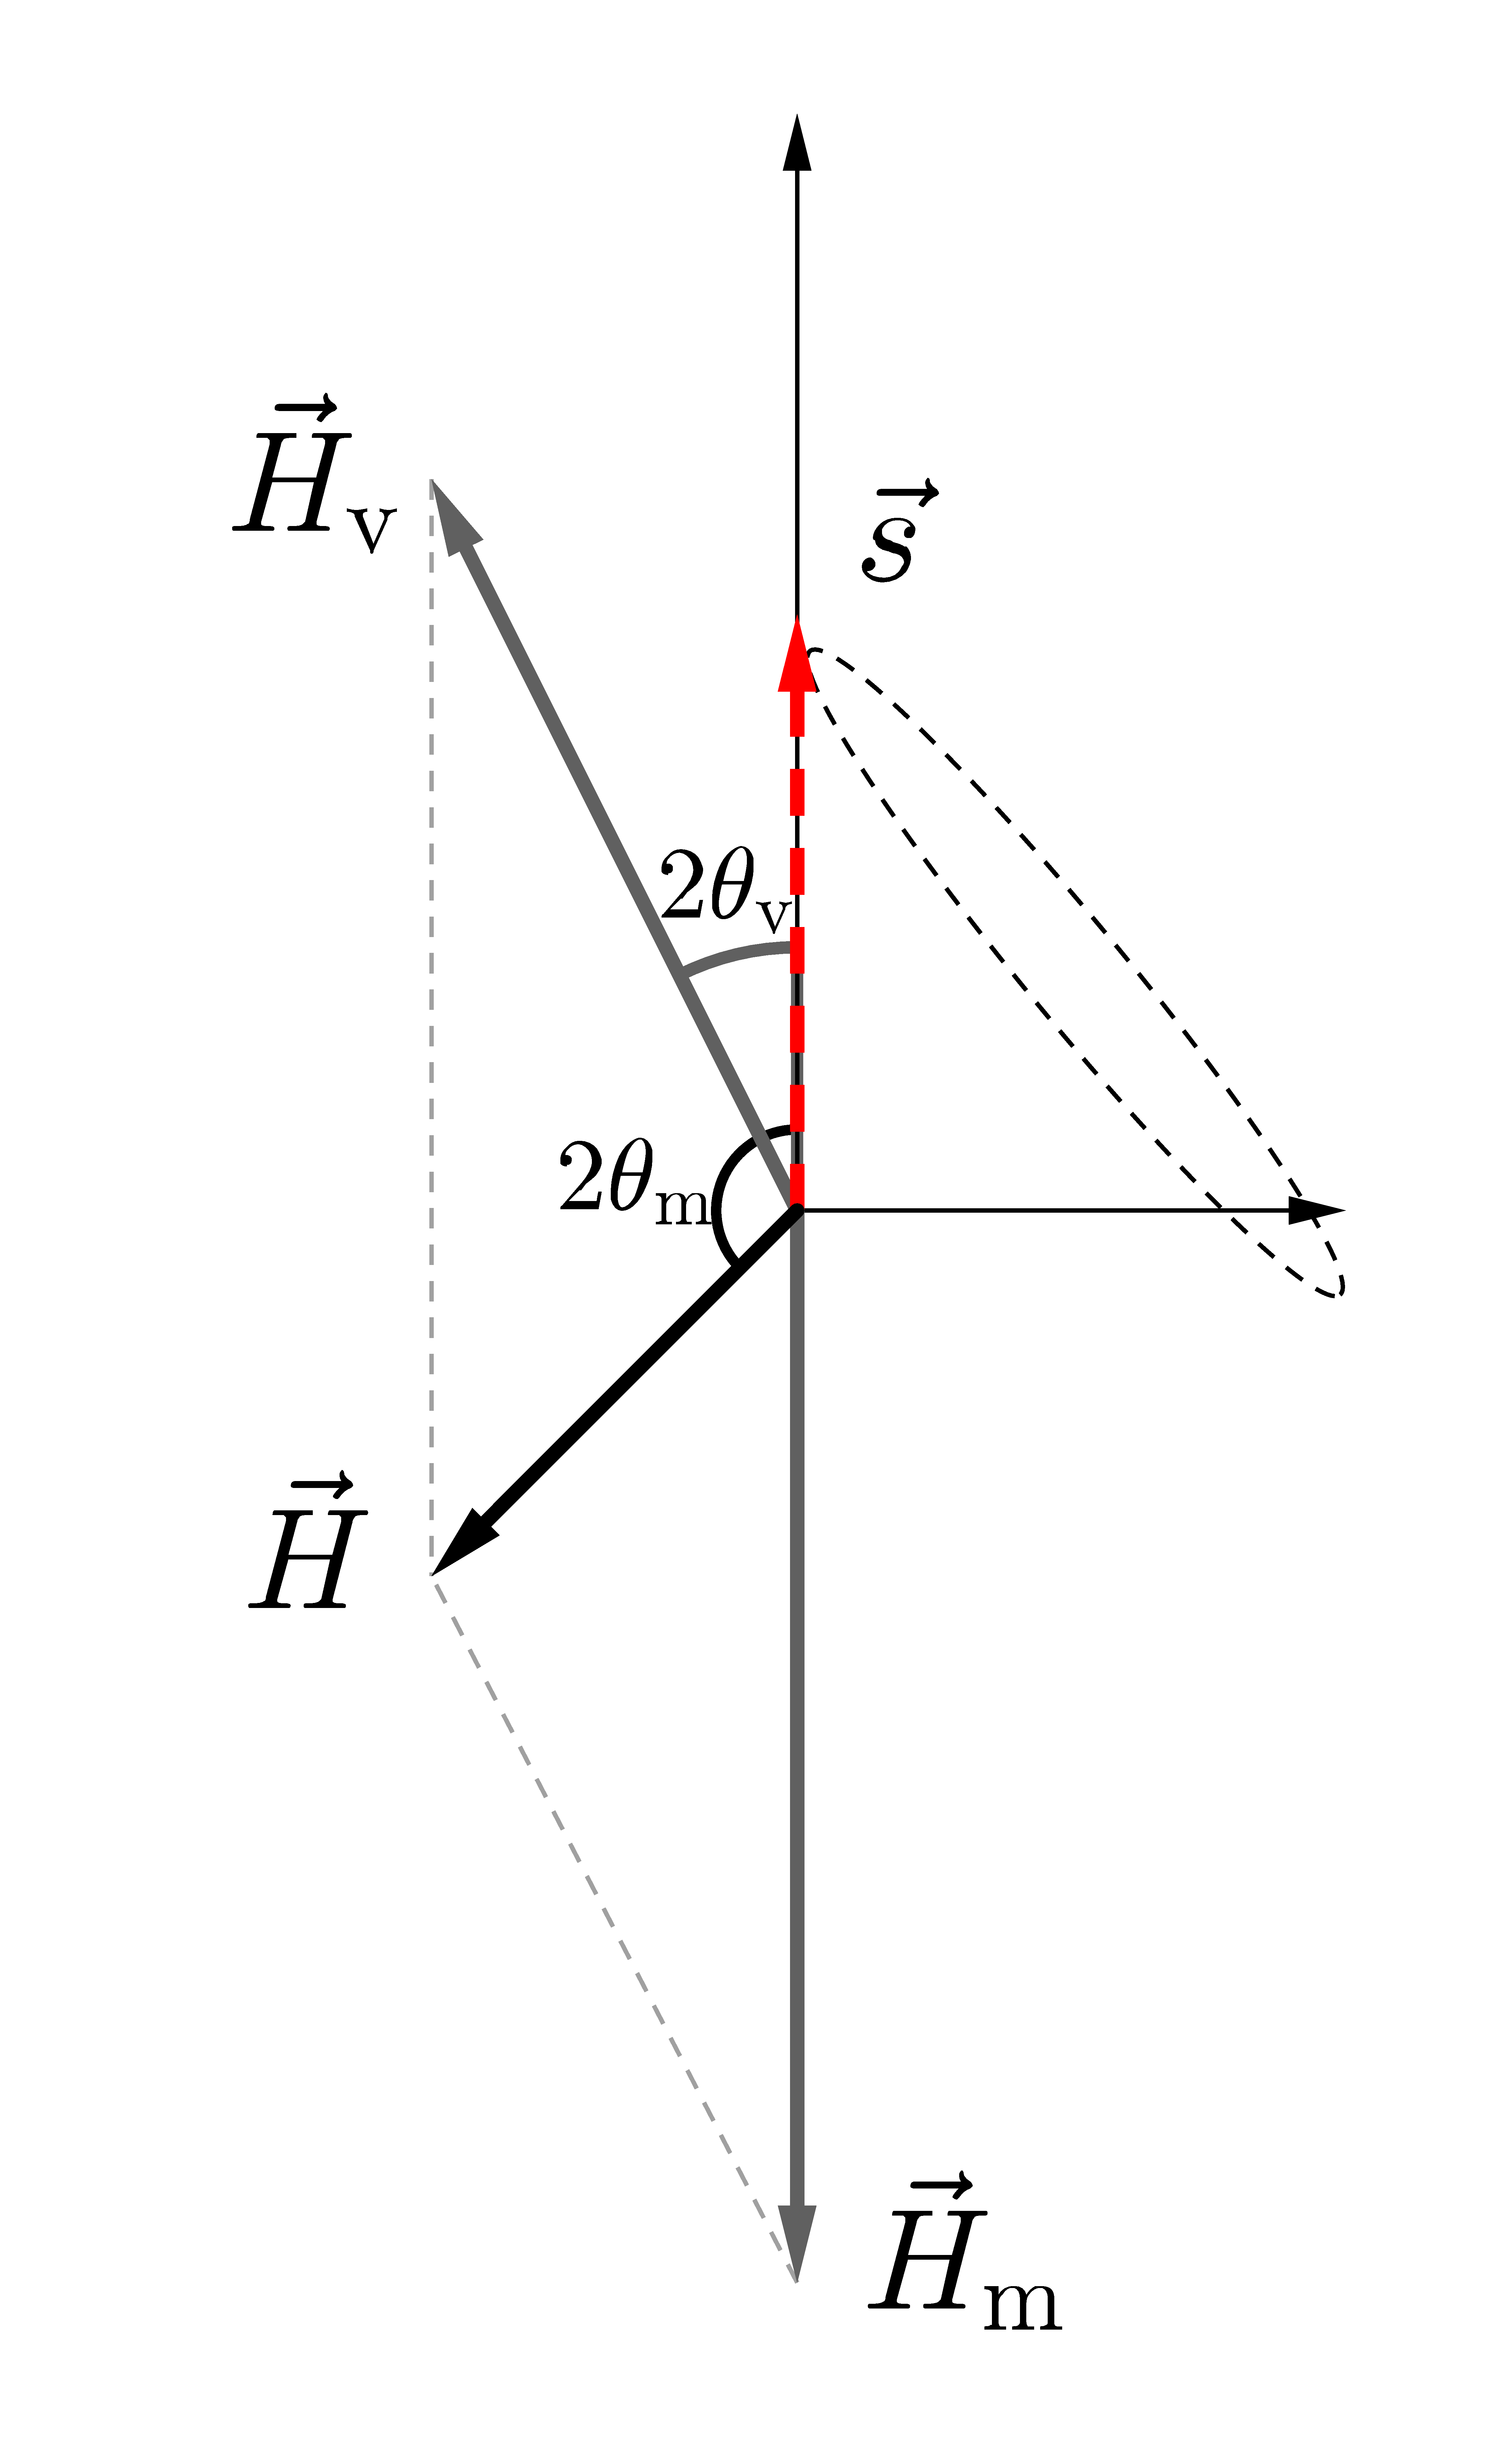
\includegraphics[width=0.4\textwidth]{chapters/assets/matter/matter-effect-notsolarge-density}
    \caption{Neutrino oscillations in flavor isospin picture, with the presence of matter potential. The flavor isospin is denoted as red dashed arrow. It starts from electron flavor. The two gray vectors stand for the Hamiltonians of vacuum $\vec H_{\mathrm v}$ and matter $\vec H_{\mathrm m}$.}
    \label{chap:basics-sec:flavor-isospin-pic-fig:matter-effect-notsolarge-density}
\end{figure}










\section{\label{chap:basics-sec:flavor-isospin-pic}Flavor Isospin Formalism}


\begin{figure}
    \centering
    \vspace*{-10pt}
    \includegraphics[width=\textwidth]{chapters/assets/basics/flavor-isospin-illus}
    \caption{In the flavor isospin picture, a flavor isospin pointing upward, i.e., along the third axis in flavor space, indicates that the neutrino is in the electron flavor, while the downward direction indicates the other flavor, such as the muon flavor.}
    \label{chap:basics-sec:flavor-isospin-pic-fig:flavor-isospin-illus}
\end{figure}

The oscillations in the two flavor scenario are consequences of the Hamiltonian in this two-level quantum system. It is known that two-level quantum systems can be visualized using the Bloch sphere. In the realm of neutrino physics, the neutrino flavor isospin was introduced for such purpose~\cite{Duan2006b}. The Hamiltonian for neutrino oscillations can be reformulated into a vector form.

Every two-by-two Hermitian matrix can be expanded in the quaternian basis. For example, the Hamiltonian for neutrino oscillations in vacuum can be written as
\begin{equation}
\mathsf H^{(\ff)} = - \frac{\vec{\sigma} }{2}\cdot {\vec{H}}^{(\ff)}.
\end{equation}
I will use $\vec{}$ to denote vectors in flavor space.
Meanwhile, the flavor quantum state of the neutrino is represented by the flavor isospin, which is defined as
\begin{equation}
    \vec s^{(\ff)} = {\Psi^{(\ff)}}^{\dagger} \frac{\vec{\sigma} }{2} \Psi^{(\ff)}.
\end{equation}
As shown in Fig.~\ref{chap:basics-sec:flavor-isospin-pic-fig:flavor-isospin-illus}, the directions of the flavor isospin in flavor space tell us the flavor content of the neutrino. A flavor isospin pointing upward in flavor space, i.e., along the direction of the third axis, denotes the electron flavor by definition. In the flavor isospin formalism, the electron flavor survival probability is
\begin{equation*}
P = \frac{1}{2} + s^{{(\ff)}}_3,
\label{chap:basics-sec:flavor-isospin-pic-eqn:probability-flavor}
\end{equation*}
where $s^{(\ff)}_3$ is the third component of the flavor isospin.
Correspondingly, the equation of motion for the flavor isospin describes its precession around the vector $\vec{H}^{(\ff)}$,
\begin{equation}
\dot{\vec{s}}^{(\ff)} = {\vec{s}}^{(\ff)} \times \vec{H}^{(\ff)}.
\label{chap:basics-sec:flavor-isospin-pic-eqn:eom-precession}
\end{equation}
This precession corresponds to periodic oscillations between the two neutrino flavors. For example, in vacuum oscillations, the Hamiltonian becomes
\begin{align*}
{\mathsf H}^{(f)} \to &\frac{\omega_{\mathrm v} }{2}\left( - \cos 2\theta_{\mathrm v } \sigma_3  + \sin 2\theta_{\mathrm{v}} \sigma_1 \right)
\to  \omega_\vv\begin{pmatrix}
 \sin \theta_\vv\\
0\\
\cos 2\theta_{\mathrm v}
\end{pmatrix},
\end{align*}
which is a vector of length $\omega_{\mathrm v}$ and tilted away from the third axis by the angle $2\theta_{\mathrm v}$.

\begin{figure}
    \centering
    \vspace*{-20pt}
    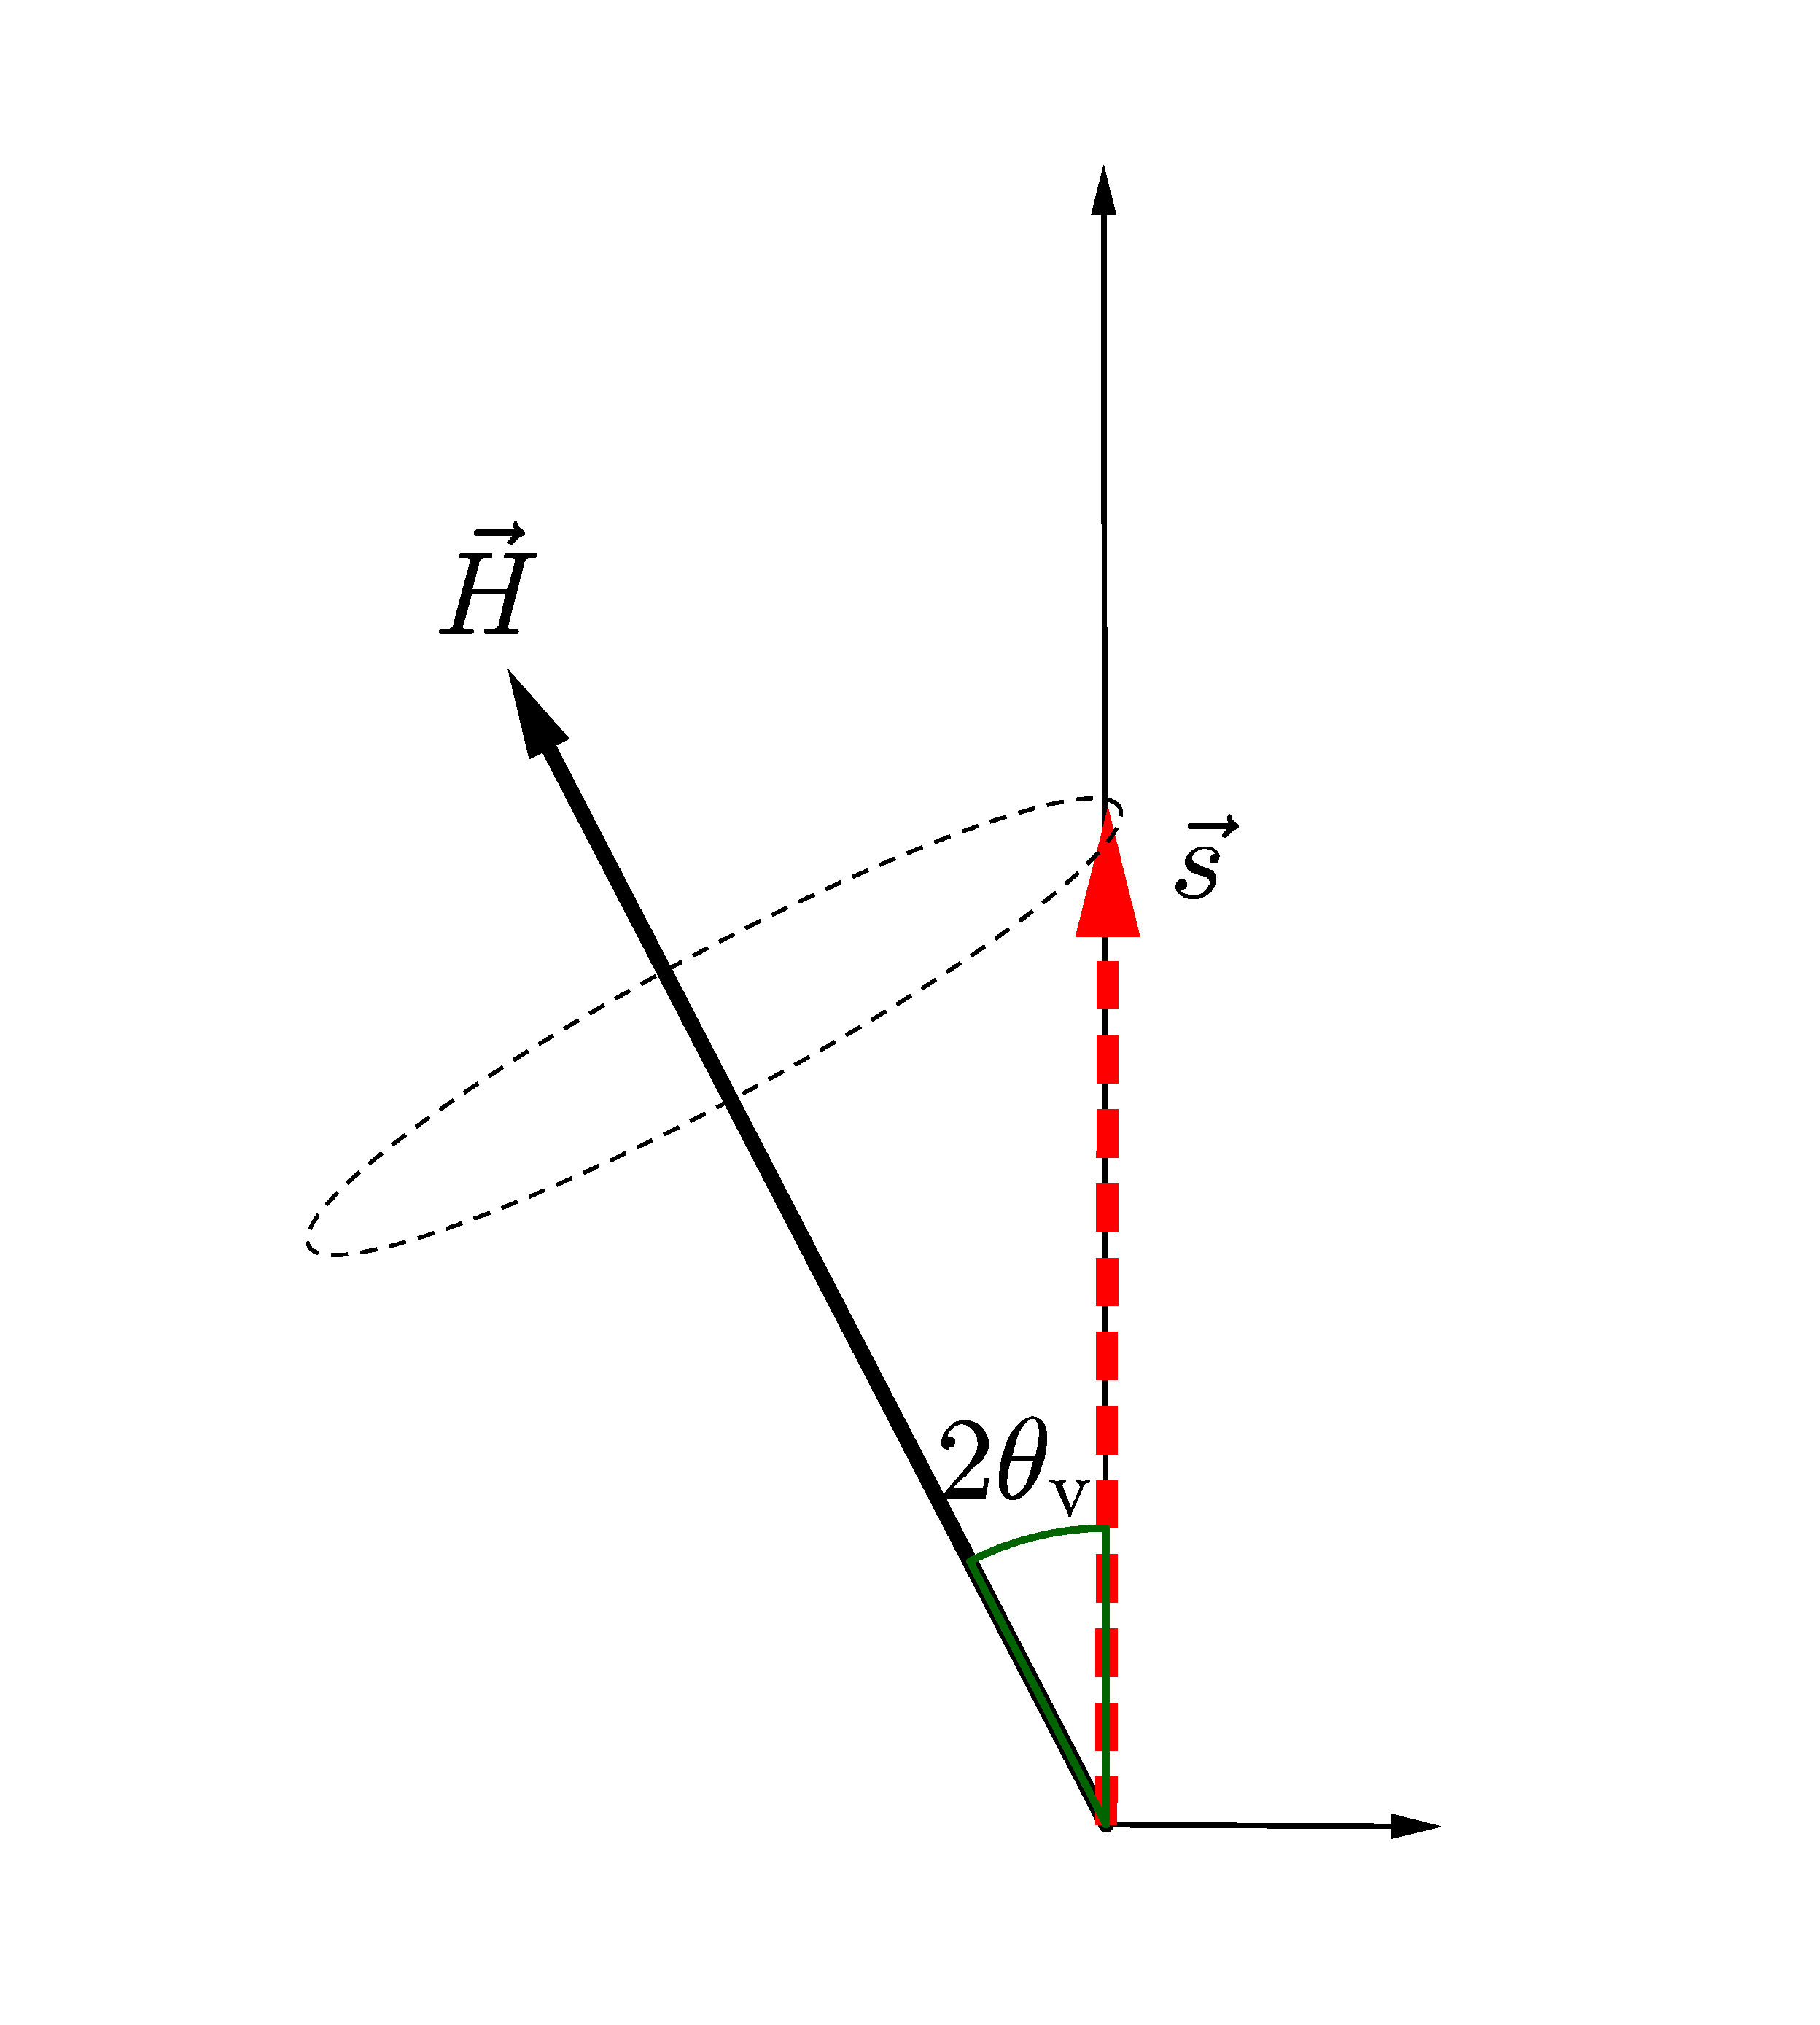
\includegraphics[width=0.6\textwidth]{chapters/assets/basics/flavor-isospin-vac-osc}
    \caption{Vacuum oscillations in the flavor isospin picture. The flavor isospin of a neutrino starting with the electron flavor will precess around the static ``Hamiltonian vector" $\vec H$, which gives periodic flavor oscillations according to Eqn.~\ref{chap:basics-sec:flavor-isospin-pic-eqn:probability-flavor}.}
    \label{chap:basics-sec:flavor-isospin-pic-fig:flavor-isospin-vac-osc}
\end{figure}

Eqn.~\ref{chap:basics-sec:flavor-isospin-pic-eqn:eom-precession} depicts the precession of the flavor isospin for a neutrino which starts with the electron flavor and propagates in vacuum. The oscillation frequency is trivially read out from Eqn.~\ref{chap:basics-sec:flavor-isospin-pic-eqn:eom-precession},
\begin{equation}
\omega_\vv = \lvert \vec{H}^{(\ff)} \rvert
\end{equation}





MSW effect is also easily explained using flavor isospin picture. The Hamiltonian in flavor isospin picture
\begin{align*}
    \mathsf H = & \frac{\omega_{\mathrm{v}}}{2}\left( - \cos 2\theta_{\mathrm{v}} {\sigma_3} + \sin 2\theta_{\mathrm{v}} {\sigma_1} \right)   + \frac{\lambda(x)}{2} {\sigma_3} \\
    \to &  \omega_{\mathrm v}\begin{pmatrix}
    - \sin 2\theta_{\mathrm v} \\
    0 \\
    \cos 2\theta_{\mathrm v}
    \end{pmatrix}   + \begin{pmatrix}
    0\\
    0\\
    - \lambda(x)
    \end{pmatrix}  \\
    = &  \vec H_{\mathrm v} + \vec H_{\mathrm m}(x),
\end{align*}
where $\vec H_{\mathrm v}$ is vacuum contribution and $\vec H_{\mathrm m}(x)$ is the matter potential contribution. The two vectors are visualized in Fig.~\ref{chap:basics-sec:flavor-isospin-pic-fig:matter-effect-notsolarge-density}. We discussed in Sec.~\ref{chap:basics-sec:msw} the adiabatic transitions of neutrino states in varying matter density. Fig.~\ref{chap:basics-sec:flavor-isospin-pic-fig:msw-adiabatic} shows the adiabatic evolution of neutrino flavor isospin. For region of high density matter background, which provides large matter potential, the total Hamiltonian is almost pointing downward. We observe almost no flavor oscillations since flavor isospin precession is tiny. As the neutrinos moving into smaller matter density regions, the flavor isospin is approximately following the evolution of Hamiltonian. Flavor conversion happens because of the evolution of Hamiltonian, even though flavor oscillations are still tiny. In the end, neutrinos reach the region with almost no matter, where they are almost converted to one of the mass eigenstates. In fact, those neutrinos won't oscillate that much in vacuum following this initial condition.






\begin{figure}[htbp]
	\centering
	\begin{subfigure}[t]{0.3\textwidth}
		\centering
		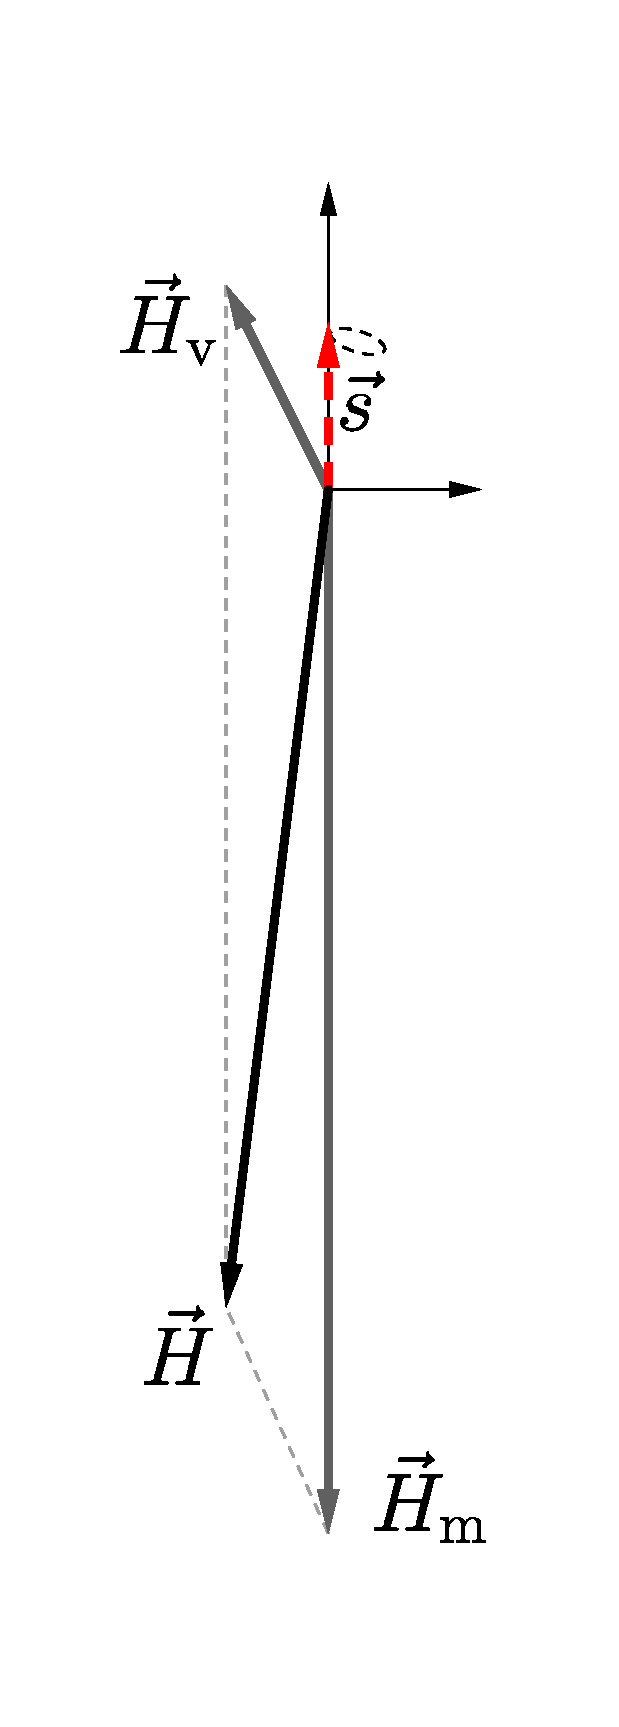
\includegraphics[width=0.8\textwidth]{chapters/assets/matter/matter-effect-large-density}
		\caption{High matter density}\label{chap:basics-sec:flavor-isospin-pic-fig:msw-adiabatic-large-density}
	\end{subfigure}
	\quad
	\begin{subfigure}[t]{0.3\textwidth}
		\centering
		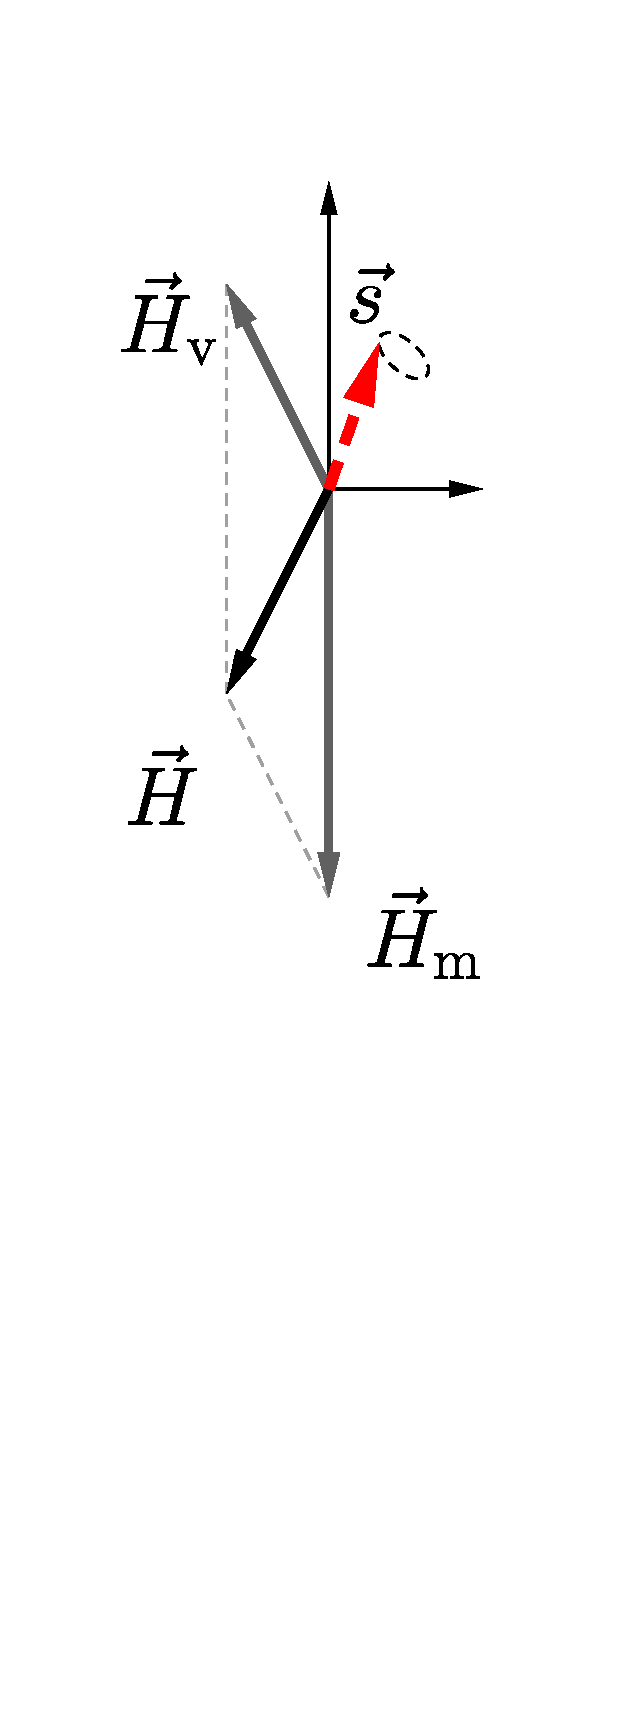
\includegraphics[width=0.8\textwidth]{chapters/assets/matter/matter-effect-adiabatic}
		\caption{Medium matter density}\label{chap:basics-sec:flavor-isospin-pic-fig:msw-adiabatic-medium-density}
	\end{subfigure}
	\quad
	\begin{subfigure}[t]{0.3\textwidth}
		\centering
		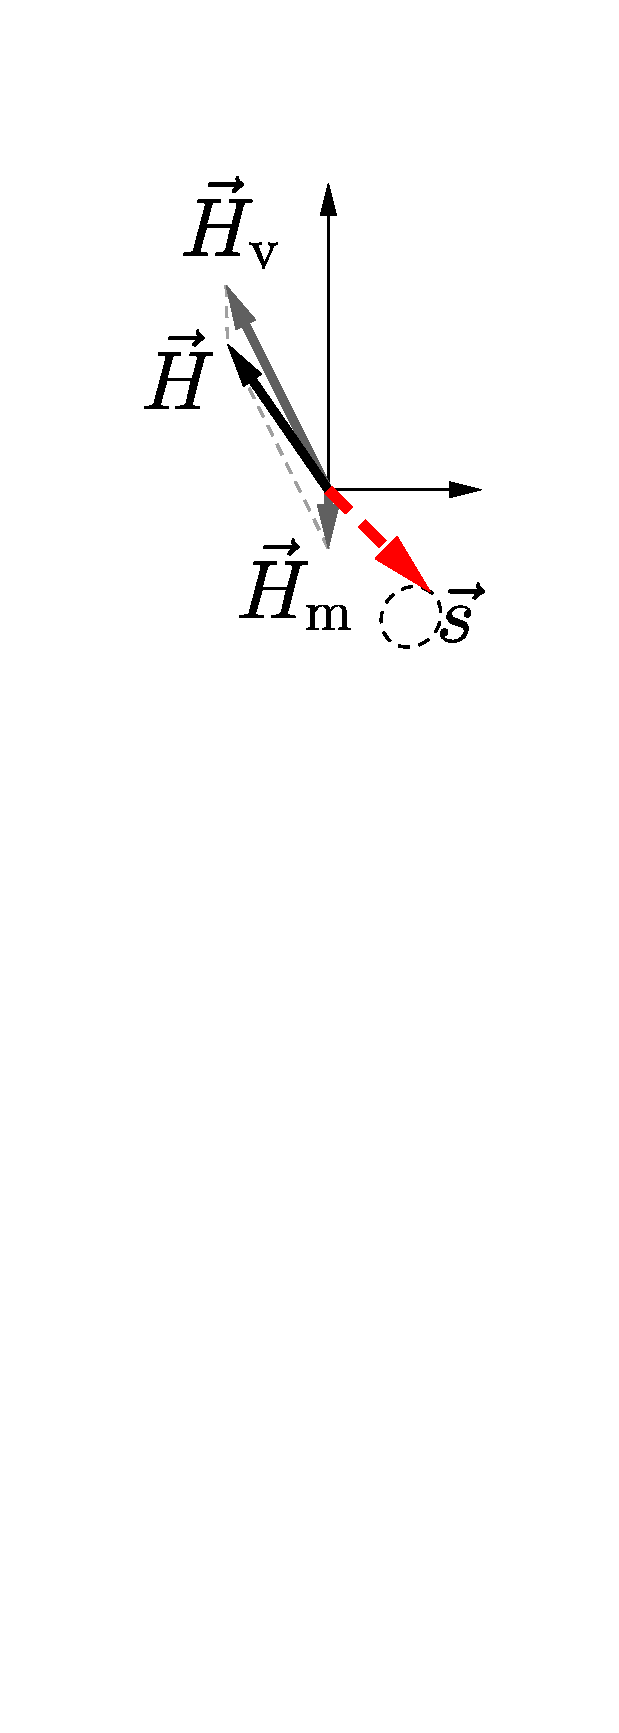
\includegraphics[width=0.8\textwidth]{chapters/assets/matter/matter-effect-adiabatic-3}
		\caption{Low matter density}\label{chap:basics-sec:flavor-isospin-pic-fig:msw-adiabatic-small-density}
	\end{subfigure}
	\caption{Flavor isospin picture of neutrino oscillations in matter. $\vec H_{\mathrm v}$ is the vacuum contribution to Hamiltonian, and $\vec H_{\mathrm m}$ corresponds to the matter potential.}\label{chap:basics-sec:flavor-isospin-pic-fig:msw-adiabatic}
\end{figure}

Neutrinos might experience a critical matter density, when the overall Hamiltonian is perpendicular to the upright axis. Assuming we have electron neutrinos going through such regions, they will experience maximum flavor oscillations, c.f.~Fig.~\ref{chap:basics-sec:flavor-isospin-pic-fig:msw-adiabatic-critical}.

\begin{figure}
    \centering
    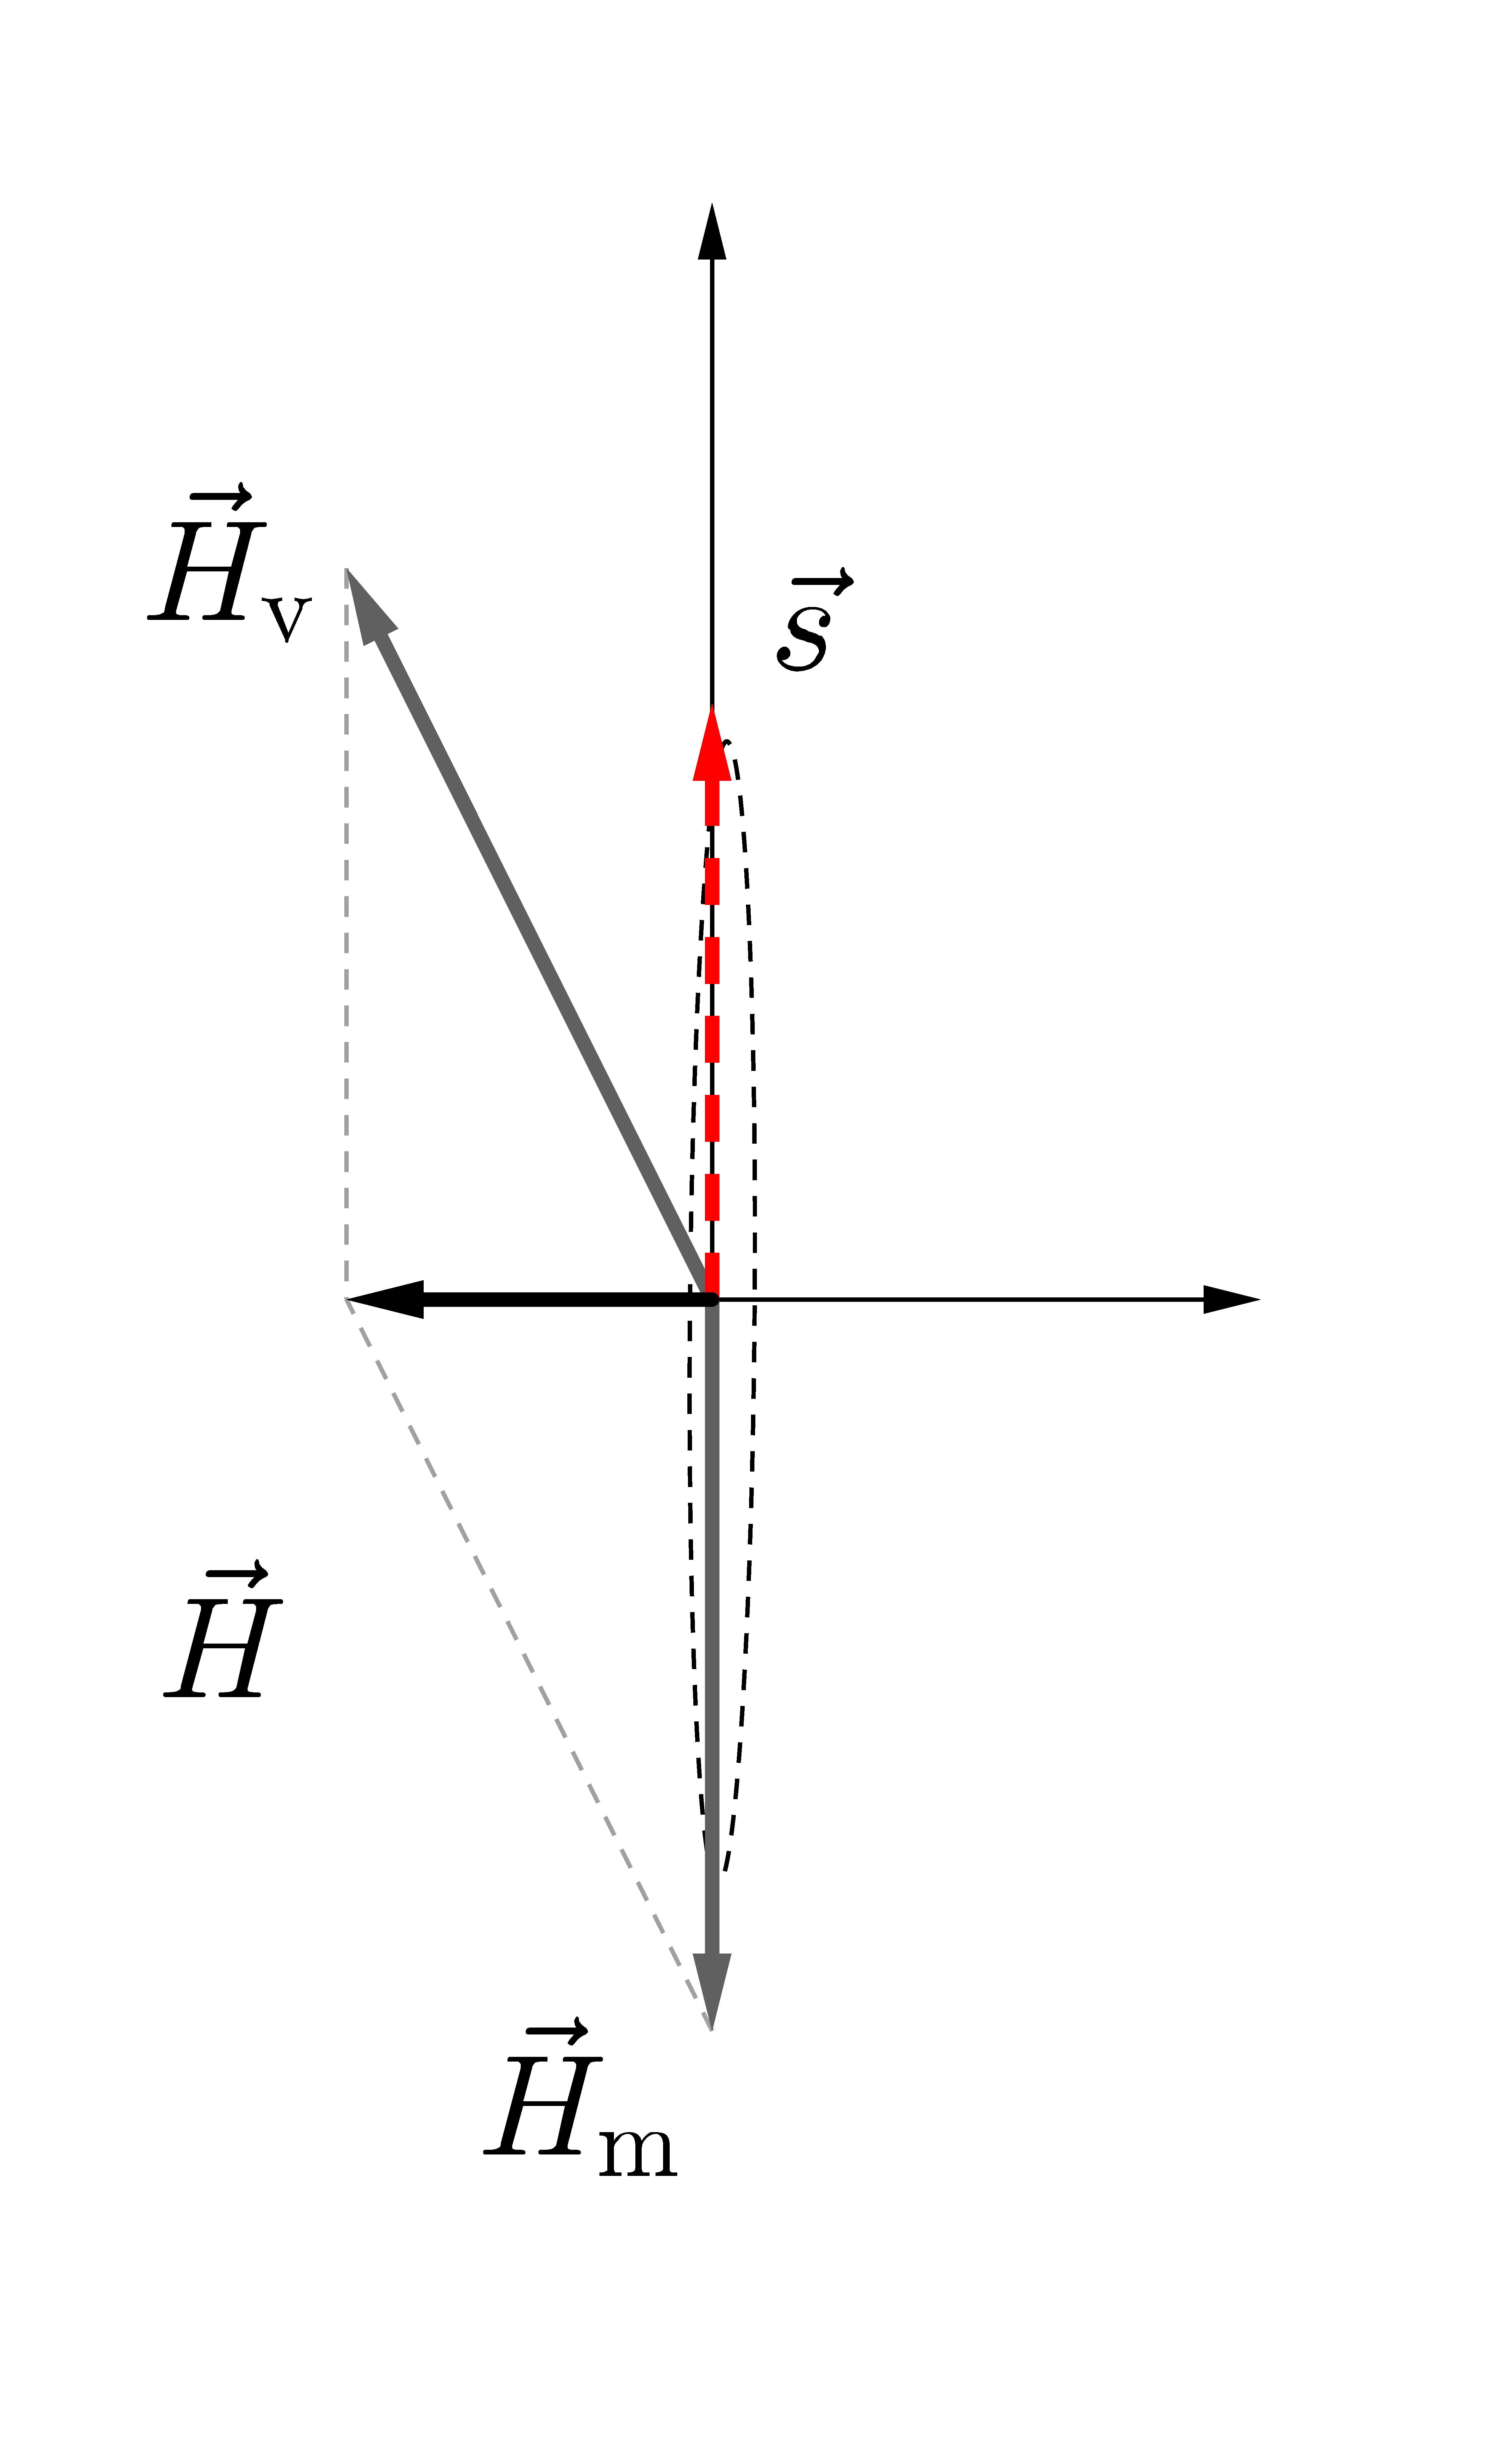
\includegraphics[width=0.5\textwidth]{chapters/assets/basics/matter-effect-critical-density}
    \caption{MSW resonance happens when electron neutrinos go through a critical matter density.}
    \label{chap:basics-sec:flavor-isospin-pic-fig:msw-adiabatic-critical}
\end{figure}






\section{Summary}

Vacuum neutrino oscillations can be easily explained and calculated. However, it conveys the message of the nature of neutrino oscillations. Neutrinos are usually produced in flavor states through weak interactions. The neutrino does not remain in the same flavor state during its propagation because the flavor states are not the eigenstates of the propagation Hamiltonian. An extrapolation of this idea is that neutrinos might also oscillate in a uniform linear potential, the Hamiltonian of which would be similar to vacuum Hamiltonian but with different values. One of such situations is that neutrinos propagate through a region with a constant matter density, which I will explain in the next chapter.
